




%\raggedleft
%\textit{
%Cet hiver a des airs de printemps\\
%Des peuples ou de l'esprit, au diable l'âme.\\
%Le vent se lève, ça faisait longtemps\\
%Triste de s'enfermer pour quelques grammes.\\
%}

%\medskip

%\raggedright

%Cet avenir des airs de passé\\
%S'il fallait juste trouver le régime,\\
%Assassinée la complexité\\
%Maintes perspectives se cachent en les crimes.\\

%\medskip
%\raggedleft

%Pour une morphogenèse politique\\
%Adieu le coron, ses tristes briques\\
%Murs qui s'érigent tuent votre espérance.\\

%\medskip
%\raggedright

%Perle de la mer, sirène hante la crique\\
%Du haut des tours s'amuser du cirque\\
%L'hiver d'idées qui peuple la France.\\




%------------------------------------


\newpage






%\chapter*{Conclusion}{Conclusion}
\chapter*{Conclusion}


% to have header for non-numbered introduction
\markboth{Conclusion}{Conclusion}


\headercit{Explorer sans relâche les systèmes géographiques\ldots}{Arnaud Banos}{}



Le lecteur qui aura tenu jusqu'ici et qui a la mémoire solide ou bien sélective, ou encore qui aura adopté un style de lecture roman policier, se plaindra du manque d'originalité dans l'origine des citations introductives. Ce n'est pas anodin si les positions de \noun{Banos}, simples mais efficaces et profondes, ouvrent et ferment ce travail : les ``9 principes de Banos'' sont implicitement présents dans la majorité des travaux menés et perspectives ouvertes. Même si une application idéale de ces principes relèverait d'un ``Démon de Banos'', à l'instar du Demon de Laplace ou de Maxwell, qui serait capable d'articuler interdisciplinaire et disciplinaire sans se perdre tout en respectant l'ensemble des principes, leur appréhension comme utopie scientifique, naturellement réflexive donc évolutive et adaptive, nous semble une entrée puissante pour de nouvelles approches intégratives des systèmes territoriaux. 

Notre contribution épistémologique, méthodologique en lien avec ces points est essentielle, même si celle ci est difficile à expliciter et nécessitera un certain recul pour être effectivement cernée. D'une certaine manière, nous avons apporté une brique supplémentaire comme \emph{proof-of-concept} du système de principes banosien, mais également comme implémentation et approfondissement de celui-ci sur certains points.



Notre contribution thématique est également difficile à situer et nécessitera un recul considérable pour appréhender ses implications. Avons-nous résolu le noeud gordien de la co-évolution ? L'avons-nous tranché ? La réponse la plus fidèle serait que nous en avons tranché une partie, celle naïve comprenant la définition dont nous sommes partis ou les positionnement de type ``poule-et-oeuf'', mais que nous avons noué une autre bien plus considérable.

















%%%%%%%%%%%%%%%%%%%%
%% Add epilogue -> may be separated




%\chapter{When Science meets Art}{Quand la science se mêle à l'art} % Chapter title

%\label{app:art} % For referencing the chapter elsewhere, use \autoref{ch:name} 

%----------------------------------------------------------------------------------------


%\includegraphics[angle=90]{Figures/Art/Capture d’écran 2016-08-08 à 11.46.55}


\begin{figure}
	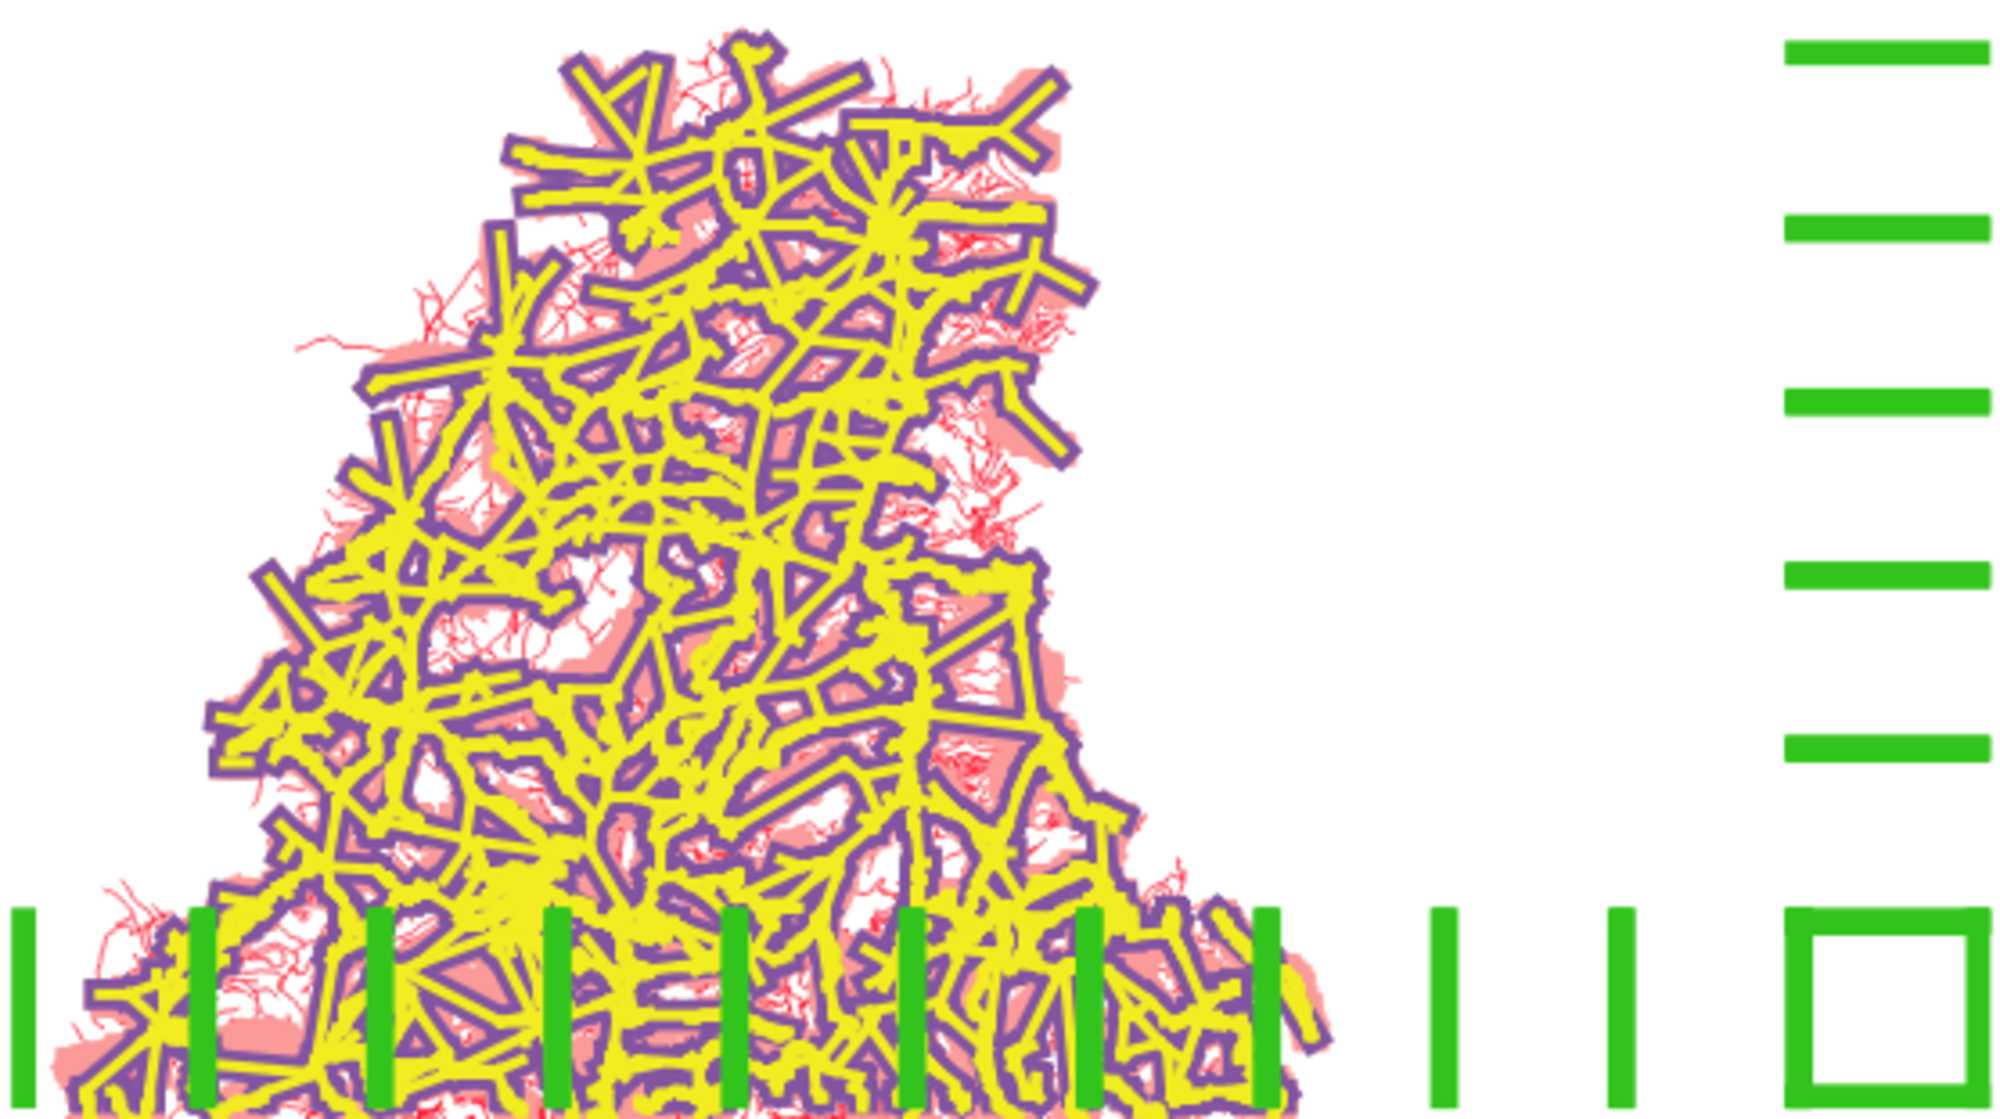
\includegraphics[width=\textheight,angle=90]{Figures/Final/CL-artwork.jpg}
\end{figure}











